%%%%%%%%%%%%%%%%%%%%%%%%%%%%%%%%%%%%%%%%%
% Arsclassica Article
% LaTeX Template
% Version 1.1 (10/6/14)
%
% License:
% CC BY-NC-SA 3.0 (http://creativecommons.org/licenses/by-nc-sa/3.0/)
%
%%%%%%%%%%%%%%%%%%%%%%%%%%%%%%%%%%%%%%%%%

%----------------------------------------------------------------------------------------
%	PACKAGES AND OTHER DOCUMENT CONFIGURATIONS
%----------------------------------------------------------------------------------------

\documentclass[
	12pt, % Main document font size
	a4paper, % Paper type, use 'letterpaper' for US Letter paper
	oneside, % One page layout (no page indentation)
	% twoside, % Two page layout (page indentation for binding and different headers)
	headinclude, footinclude, % Extra spacing for the header and footer
	BCOR5mm, % Binding correction
]{scrartcl}


%%%%%%%%%%%%%%%%%%%%%%%%%%%%%%%%%%%%%%%%%
% Arsclassica Article
% Structure Specification File
%
% This file has been downloaded from:
% http://www.LaTeXTemplates.com
%
% Original author:
% Lorenzo Pantieri (http://www.lorenzopantieri.net) with extensive modifications by:
% Vel (vel@latextemplates.com)
%
% License:
% CC BY-NC-SA 3.0 (http://creativecommons.org/licenses/by-nc-sa/3.0/)
%
%%%%%%%%%%%%%%%%%%%%%%%%%%%%%%%%%%%%%%%%%

%----------------------------------------------------------------------------------------
%	REQUIRED PACKAGES
%----------------------------------------------------------------------------------------

\usepackage[
nochapters, % Turn off chapters since this is an article
beramono, % Use the Bera Mono font for monospaced text (\texttt)
eulermath,% Use the Euler font for mathematics
pdfspacing, % Makes use of pdftex’ letter spacing capabilities via the microtype package
dottedtoc, % Dotted lines leading to the page numbers in the table of contents
%author-year
%abbrvnat % use natbib?
]{classicthesis} % The layout is based on the Classic Thesis style

\usepackage{arsclassica} % Modifies the Classic Thesis package

% \usepackage{lmodern} % Modifies the Latin Modern font

\usepackage{soul}

\usepackage[T1]{fontenc} % Use 8-bit encoding that has 256 glyphs

\usepackage[utf8]{inputenc} % Required for including letters with accents

\usepackage{graphicx} % Required for including images

\graphicspath{{./}} % Set the default folder for images

\usepackage{enumitem} % Required for manipulating the whitespace between and within lists

\usepackage{lipsum} % Used for inserting dummy 'Lorem ipsum' text into the template

\usepackage{subfig} % Required for creating figures with multiple parts (subfigures)

\usepackage{amsmath,amssymb,amsthm} % For including math equations, theorems, symbols, etc

\usepackage{varioref} % More descriptive referencing

%\usepackage[style=ieee]{biblatex}
\usepackage[authoryear,round,colon]{natbib}
\bibpunct{(}{)}{;}{autheryear}{,}{;}

%----------------------------------------------------------------------------------------
%	GANTT
%---------------------------------------------------------------------------------------


%\usepackage{tikz}
%\usepackage{gantt}
%\usepackage{pgfgantt}

%\usepackage{geometry} % to change margins
%\usepackage{pdflscape} % provides the landscape environment
%\usepackage{ragged2e} % provides \RaggedLeft


%----------------------------------------------------------------------------------------
%	break url
%---------------------------------------------------------------------------------------
% \usepackage[hyphens]{url}
\usepackage{hyperref}
\def\UrlBreaks{\do\/\do-}


%----------------------------------------------------------------------------------------
%	LANDSCAPE TABLE
%---------------------------------------------------------------------------------------
\usepackage[a4paper,left=3cm,right=3cm,top=3.0cm,bottom=3.0cm]{geometry}
\usepackage{pdflscape}


%----------------------------------------------------------------------------------------
%	THEOREM STYLES
%---------------------------------------------------------------------------------------

\theoremstyle{definition} % Define theorem styles here based on the definition style (used for definitions and examples)
\newtheorem{definition}{Definition}

\theoremstyle{plain} % Define theorem styles here based on the plain style (used for theorems, lemmas, propositions)
\newtheorem{theorem}{Theorem}

\theoremstyle{remark} % Define theorem styles here based on the remark style (used for remarks and notes)

%----------------------------------------------------------------------------------------
%	HYPERLINKS
%---------------------------------------------------------------------------------------

\hypersetup{
%draft, % Uncomment to remove all links (useful for printing in black and white)
colorlinks=true, breaklinks=true, bookmarks=true, bookmarksnumbered,
urlcolor=webbrown, linkcolor=RoyalBlue, citecolor=webgreen, % Link colors
pdftitle={}, % PDF title
pdfauthor={\textcopyright}, % PDF Author
pdfsubject={}, % PDF Subject
pdfkeywords={}, % PDF Keywords
pdfcreator={Pirchiner.co}, % PDF Creator
pdfproducer={Pirchiner.co} % PDF producer
}
 % Include the structure.tex file which specified the document structure and layout
\DeclareGraphicsExtensions{.pdf,.png,.jpg}

\hyphenation{Fortran hy-phen-ation} % Specify custom hyphenation points in words with dashes where you would like hyphenation to occur, or alternatively, don't put any dashes in a word to stop hyphenation altogether

%----------------------------------------------------------------------------------------
%	TITLE AND AUTHOR(S)
%----------------------------------------------------------------------------------------

% The article title
\title{\LARGE{
	Semantics of the Anthropocene:\\
	(towards a big) history ontology,\\
	(for machine) learning and reasoning\\
	(applied) for governance and sustainability
}}

% The article author(s) - author affiliations need to be specified in the AUTHOR AFFILIATIONS block
\author{\spacedlowsmallcaps{
	Marlon Pirchiner\textsuperscript{1,2}}
}

% An optional date to appear under the author(s)
\date{\small{\textbf{
	Preliminary Research Plan}\\
	October, 2016}
}

%----------------------------------------------------------------------------------------
\begin{document}

%----------------------------------------------------------------------------------------
%	HEADERS
%----------------------------------------------------------------------------------------

\renewcommand{\sectionmark}[1]{\markright{\spacedlowsmallcaps{#1}}}
% The header for all pages (oneside) or for even pages (twoside)
%\renewcommand{\subsectionmark}[1]{\markright{\thesubsection~#1}}
% Uncomment when using the twoside option - this modifies the header on odd pages
\lehead{\mbox{\llap{\small\thepage\kern1em\color{halfgray} \vline}\color{halfgray}\hspace{0.5em}\rightmark\hfil}} % The header style

\pagestyle{scrheadings} % Enable the headers specified in this block

%----------------------------------------------------------------------------------------
%	TABLE OF CONTENTS & LISTS OF FIGURES AND TABLES
%----------------------------------------------------------------------------------------

\maketitle % Print the title/author/date block

\setcounter{tocdepth}{2} % Set the depth of the table of contents to show sections and subsections only

\tableofcontents % Print the table of contents
% \listoffigures % Print the list of figures
% \listoftables % Print the list of tables

%----------------------------------------------------------------------------------------
%	ABSTRACT
%----------------------------------------------------------------------------------------

% This section will not appear in the table of contents due to the star (\section*)

\section*{Abstract}

	This preliminary research plan is about to taking an approach from Information Sciences and Semantic Web \citep{tim_berners-lee_james_hendler_and_ora_lassila_semantic_2001} to identify, conceptualize and model real knowledge about the Anthropocene \citep{crutzen_anthropocene_2000}, including the general notion of the time, the Geological Time Scale \citep{gradstein_geologic_2004}, the International Chronostratigraphic Chart \citep{cohen_ics_2013} and others. If successful, a natural extention could be evaluate social models \citep{pitt_interleaving_2011} for social and environmental applications, or governance and sustainability \citep{patterson_exploring_2016} towards a \citep{buckingham_shum_towards_2012}. For a concrete example, the \citep{icsu-issc_review_2015} sustainable outcomes for \citep{united_nations_transforming_2015} agenda for 2030 in sustainable development could be modeled and monitored by semantic scientific workflows using ontologies built for Anthropocene and Big-History supported by linked and open data.

%Starting in 1950 the Anthropocene can be understood as the exponential growing behavior in some fundamental socio-environmental indicators. To compose that indicators is used informations and data coming from many scientific domains.

%Considering specially those related to the environment and those about the human socio cultural dimension there is a huge amount of data, terms, concepts and informations related to describe and model some of our activities

%The main focus of this research proposal is to study the scientific contributions for the life conditions improvement during Anthropocene. The pathway chosen for that is to strongly consider populations and their relations with the environment through their economical and cultural practices materialized into public policies and regulations stablished over territories by their internal and external dynamic flows.

%\begin{enumerate}
%\item Which collective actions, if adopted, could have the most impact for future sustainability and social happiness?
%\item Are the existent ontologies, vocabularies and semantic technologies, models and workflows helpful in a decision making and governance process?
%\end{enumerate}

%----------------------------------------------------------------------------------------
%	AUTHOR AFFILIATIONS
%----------------------------------------------------------------------------------------

{\let\thefootnote\relax\footnotetext{\textsuperscript{1}\textit{
Previously at Department of Geophysics, Institute of Astronomy, Geophysics and Atmospherical Sciences - IAG, University of São Paulo - USP, São Paulo, Brazil}}}

{\let\thefootnote\relax\footnotetext{\textsuperscript{2}\textit{
Formerly at Applied Math School - EMAp, Getúlio Vargas Foundation - FGV, Rio de Janeiro, Brazil
}}}

%----------------------------------------------------------------------------------------
\newpage
% Start the article content on the second page, remove this if you have a longer abstract that goes onto the second page

%----------------------------------------------------------------------------
% Context
%----------------------------------------------------------------------------
\section{Context}

Anthropocene \citep{crutzen_anthropocene_2000, crutzen_geology_2002} and Big History \citep{christian_maps_2004} share the unifying nature of their discourses. To achieve their goals they had to deal with and organize a huge amount of knowledge, information and data from many sources and disciplines such as Earth System sciences \citep{jacobson_earth_2000} revealing appearances of a new world \citep{zalasiewicz_new_2010}. There are many relevant subjects in Natural, Social Sciences and Humanities to consider, select, collect and monitor in order to create, for instance, the key indicators of the Anthropocene \citep{steffen_anthropocene:_2011}. All these transformations and their historical perspectives will likely be taught in Big History as well.

Roughly thinking, those recent ideas offer an unified view of a phenomena, let them be the overall passage of the time or a self similar behavior in social and natural indicators, by select and collect samples, organize them and prepare a single very detailed story. However, in which extent Big History and Anthropocene articulate the same trans-disciplinary concepts? What they tell about, for instance, the notion of time? How many reliable workflows, models, meanings, relations and data these concepts can map? If a task was to monitor and provide evidences, at proper scale and format, for governance and decision making processes, in the context of \citet{icsu-issc_review_2015} scientific perspective for a global agenda concerned to the sustainable development goals \citep{united_nations_transforming_2015}, will be these formalized concepts and relations from Big History and Anthropocene, materialized into ontologies, suitable for help?

Working by join many different knowledge domains, some common issues are often faced by researchers, such as the use of many terms or a whole tacit terminology referring to, sometimes, misleading informations and data with lack of provenance \citep{lebo_prov-o:_2013,ma_capturing_2014}. The rise of information specific subjects is a recognized scientific problem \citep{fox_rise_2012} and this have made librarians, ontologists and information engineers became absolutely necessary and required to compose multidisciplinary teams by adding their skills. They are known to be very precise on organizing the knowledge by subjects, terminologies, authors, institutions and even with the physical disposal of archives and needs for document and sampling preservations. In data and digital worlds, will not be different.

Inside and beyond Earth and Space Sciences, Anthropocene and Big History are examples of research fields where the information era took also a central place and has been largely discussed \citep{baker_egy:_2009}. Informational technologies and analytics are dominating the innovation agenda by putting `intelligence' on everything, the so called Internet of Things \citep{kopetz_internet_2011}. The reality is that some pieces as turbines, airplanes, even cellphones, almost everything are becoming sensors -- and actors. In many cases they also are able to provide realtime data streams, collecting data signatures of themselves and of the surrounding environment. They respond, in the most part of the time, to remote controls. Sometimes they are able to react automatically based on thresholds or as answer to an environmental status. Taking a look at self driven cars, trucks and drones gives a couple of concrete examples. Data streams have been flowing to the big-data ocean.

This proposal is about to take an approach from Information Sciences perspective, to development a Big History Ontology for the Anthropocene -- BHOA -- reusing, as much as possible, other available ontologies \citep{hobbs_ontology_2004,cox_formal_2005,raskin_knowledge_2005,cox_geologic_2015,cox_time_2016}. This would be used to represent models for social and natural simulations \citep{pitt_interleaving_2011} applied for governance and sustainability \citep{patterson_exploring_2016}. This is a challenging task whenever it involves the systematization of subjects and knowledge coming from many natural and social disciplines and research fields with controversial themes. There are many utilities for ontologies, but an irrefutable one is to assist on communication centric tasks such as researching, teaching, outreaching or in public awareness.

A very important goal of this doctorate proposal is, at the end, be able to use all linked, opened and available data to constraint, by semantic reasoning, social simulations investigating consequences of public regulations and agenda prioritization for the environment and next generations \citep{biermann_navigating_2012}.

%----------------------------------------------------------------------------
% Research Questions
%----------------------------------------------------------------------------
\section{Research Questions}

With BHOA ontology and instantiated data, it is expected to became possible to answer research questions about where, or in which subjects, Anthropocene and Big History have more synergy or refer to close related concepts or foundational datasets. This is also a challenging task due the tweezer proposed approach and means to take, at least, two parallel pipelines. In one side, a deductive approach from librarian and information sciences guidelines to a rational top-down ontological and theoretical effort to capture meanings and organization. On the other side, an abductive approach, taking use of natural language processing and analytics to empirically gives a bottom-up structure to unstructured data. The manifold expecting result is the ability to boost and augmenting, by semantic matching, capabilities to represent, model and solve problems by accessing at same time the conceptual world and all semantically related data, algorithms and references involved, called also as semantic e-Science \citep{narock_science_2012,ma_semantic_2015}.

By using this ontology, and all related and linked data addressed on the Web, the second group of research questions is about in which extent BHOA ontology could be used to express also models from the workflows used to compute some Anthropocene indicators or even help to build new others. Based on a high extent answer for the last questions, it is also possible to check how easy could be to found, selected and implemented those models. It might be possible to consider additional requirements such as assimilation of new observations for integrated performance monitoring or the ability to simulate and forecast future scenarios or estimating uncertainties. Much in this sense have been made by \cite{biermann_navigating_2012}.

A third and last scientific question group to answer in the course of this work is how the conjugated ability to extract, capture and expand concepts, relationships and formal constraints, in one side, and to analyze, model, express and evaluate workflows, in another, can be used together to support evidence-based governance decisions for multi scaled levels by learning from many relevant data and document sources, performing simulations and scenario optimizations \citep{pitt_axiomatization_2012}. This is a very challenging task and it is not really expected to be completed within three years timespan. In the better case a prototype could be evaluated. To perform a whole iterative development cycle, the initial idea is to consider only the first \citet{united_nations_transforming_2015} sustainable development goal, ``to eliminate the poverty'', to make a concept proof.

%----------------------------------------------------------------------------
% Methodology
%----------------------------------------------------------------------------
\section{Suggested Methodology}

Generally, there is an intention to operate a tweezer movement. From a deductive point of view, and a top-down approach, this research propose to identify, organize and encode the concepts, objects or nodes and relations, properties or edges, linked and open data \citep{berners-lee_publishing_2001,berners-lee_linked_2006,bizer_linked_2009} as well provenance \citep{lebo_prov-o:_2013} plus authorship and metadata. This work should be performed considering the authority of data providers, if peer-reviewed, and their reputations, for instance, if they are community-based. There is nothing so inventive to do not follow international standards \citep{w3c_w3c_2015} and best practices \citep{tandy_spatial_2016}.

From an abductive perspective, a bottom-up approach \citep{gil_data_2009}, the proposal is to create a pipeline for natural language processing \citep{blei_probabilistic_2012} (may be extended by translations further). The general idea is became able to structure initially unstructured data, working as a big historian in a big archive of peer-reviewed published articles grabbing information of their subjects, terminologies, concepts and hopefully extract their conceptual models, even when they involves formulas, tables, graphics or resources in any other media or sensors. There is already a solid research field supporting this path-work, for instance the Stanford group\footnote{Stanford NLP Group \url{http://nlp.stanford.edu}} to mention only one.

The analytical and synthetical movements of this research is proposed to occur working on mechanisms for matching \citep{zheng_sem+:_2015}. They are expected to be extremely useful on create value in problem solving using both approaches or perspectives. Adding value bottom-up, for instance crowdsources, sensors or augmenting people, by matching and annotating them with all additional information and links to make them discoverable and usable for further applications as monitoring, research, decision making or any other.

A standard use case which could adopted is to track all provenance, metadata, analysis methods and real data involved \cite{ma_capturing_2014} to encapsulate them into reproducible workflows \citep{mattoso_addressing_2016}. An initial idea could be to start with the visualizations of the key social and natural indicators of the Anthropocene. This can be done by manually in a training phase but automated through a semantic matching algorithm.

At the end, looking for agent based modeling, the intention is to follow \cite{pitt_interleaving_2011,pitt_axiomatization_2012} and \cite{jones_design_2013} idealistically towards a ``global democracy and Earth System governance'' \citep{dryzek_global_2011}
or a ``global participatory platform'' \citep{buckingham_shum_towards_2012} by ``democratising open data, complexity science and collective intelligence'', ``exploring the governance and politics of transformations towards sustainability''\citep{patterson_exploring_2016}.


%----------------------------------------------------------------------------
% Working Plan
%----------------------------------------------------------------------------
\section{Working Plan}

Table \ref{tab:working_plan} present a very broad and open timetable for the project development and conclusion.

% \begin{landscape}
	% \thispagestyle{empty}
	\begin{table}[h]
    \centering
  	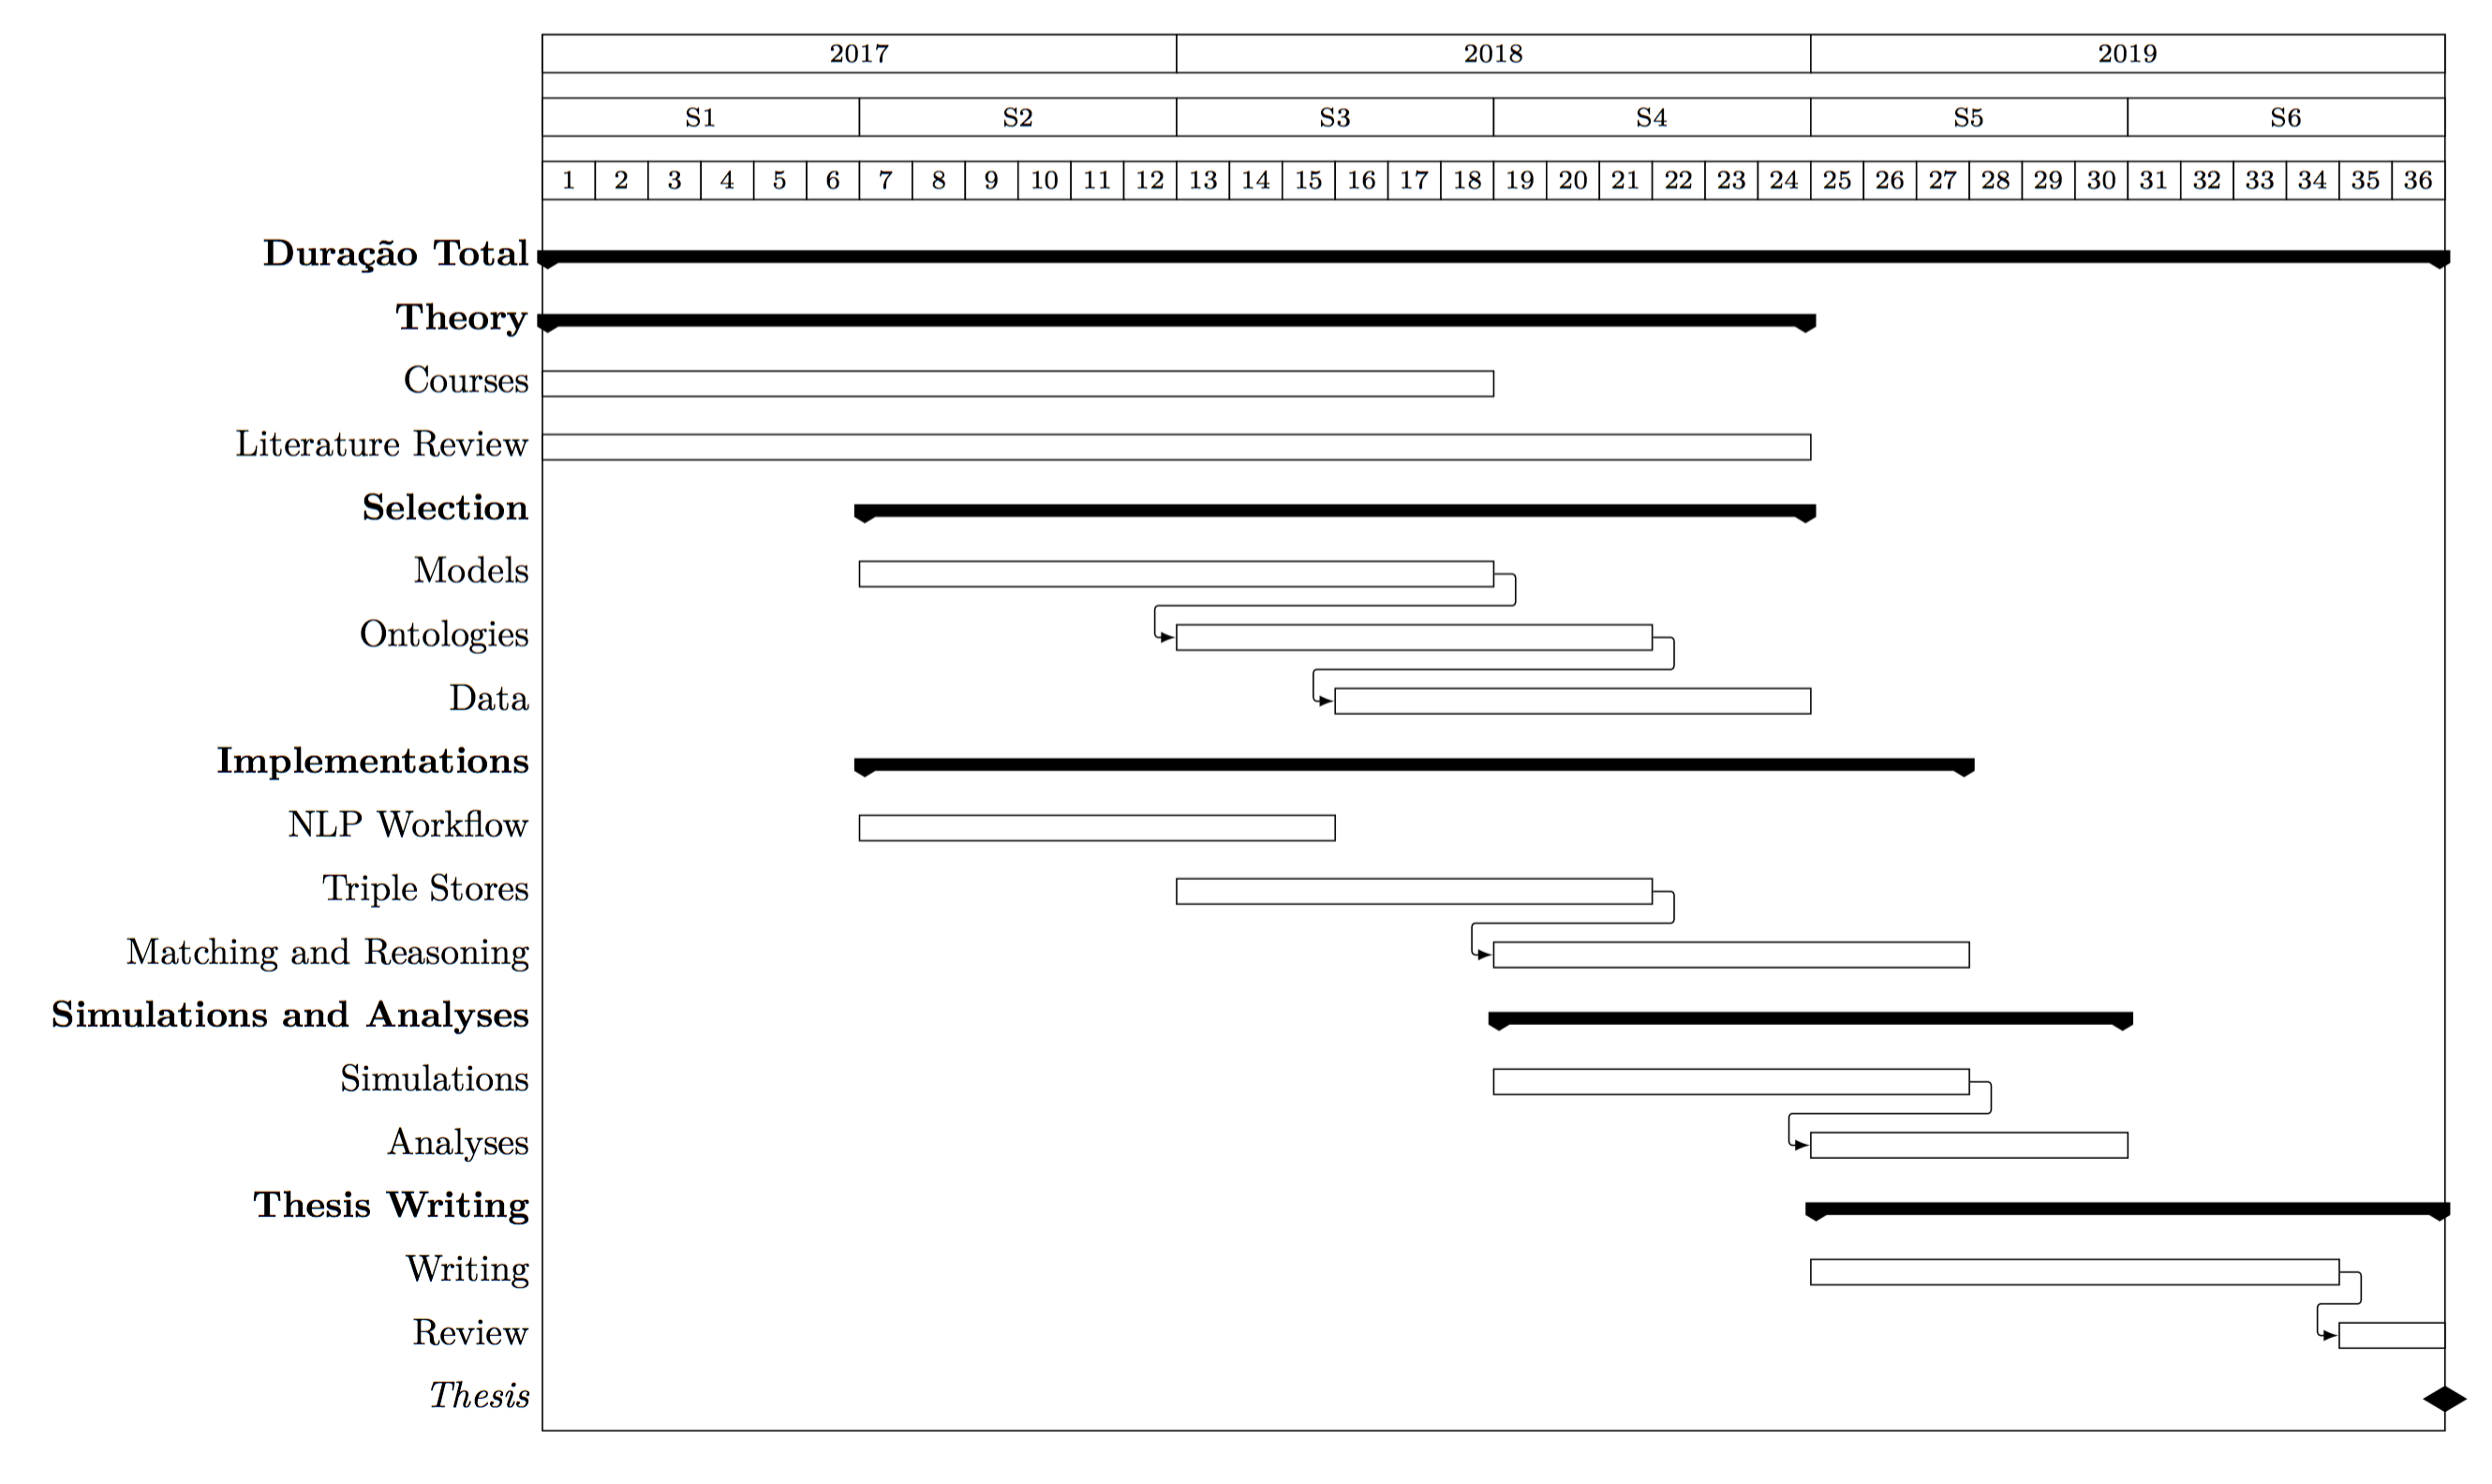
\includegraphics[width=1.00\columnwidth]{timetable_png}
		\caption[Working Plan]{Working Plan}
		% The text in the square bracket is the caption for the list of figures while the text in the curly brackets is the figure caption
		\label{tab:working_plan}
	\end{table}
% \end{landscape}

To be concluded in the timespan of three years, more than time reserved for theory, intellectual development and writing, the work plan on Table \ref{tab:working_plan} shows three other core sections. One, at the beginning, is dedicated to select models, ontologies and data. A second one, in almost same time span, is dedicated to code writing and services implementations such NPL workflow, triple stores or matching and reasoning algorithms. A last third group is about simulations and analysis. If all everything had worked well, here would be possible to analyze results from some agent-based scenario simulations.

It is important to note that this is a very broad timetable (Tab. \ref{tab:working_plan}) and could be rearranged further.

%----------------------------------------------------------------------------
%	Expected Results
%----------------------------------------------------------------------------
\section{Expected Results}

By matching entities, terminologies and vocabularies with ontologies, it could be possible to inherit formal relationships from more abstract scales or upper ontologies. By linking observations, giving them semantic meaning in the web, through ontologies would be possible to map data and the workflows responsible to reproduce results, simulate and forecast \citep{patton_semnext:_2015} or also be modified in any desired aspect. A linked data infrastructure for Big History and Anthropocene maintained aside a clear ontology based on reliable scientific content \citep{gil_towards_2007} and community standards \citep{w3c_w3c_2015} could provide a smart engine to assimilate earth observations for many applications from modeling to simulations, forecasts and visualizations.


People can discuss whenever the Anthropocene can be consider a rupture \citep{hamilton_anthropocene_2016} or just an ideology \citep{baskin_ideology_2014}. Despite if its begin is already known \citep{zalasiewicz_when_2015} or not, accepted or not \citep{zalasiewicz_anthropocene:_2011}, humans became letting more than only their footprints and this is an evidence. If the concept could be useful as Gaia \citep{lovelock_gaia_1979} to integrate and helpful to understand inter-relationships between notions and knowledge from an initially apart situation, it would be supported. At the end public policies are, in fact, issues for complex social systems \citep{furtado_complexity_2015, da_silva_territory_2015}.


%----------------------------------------------------------------------------
%	Final Considerations
%----------------------------------------------------------------------------
\section*{Final Considerations}
%

This proposal is under-construction document. At this version it only represent a couple of quickly joined intentions. It could be even more general or specific, but it has been made as a icebreaker for further research discussions.

To conclude it, I was forced to stop it in some point under the threat to still writing forever. I hope this could have been at least a little enlightening at this point.


%----------------------------------------------------------------------------------------
%	BIBLIOGRAPHY
%----------------------------------------------------------------------------------------

% For modifying the bibliography heading
\renewcommand{\refname}{\spacedlowsmallcaps{References}}

%\bibliographystyle{unsrt}
\bibliographystyle{plainnat}
\bibliography{phd.bib} % The file containing the bibliography

%----------------------------------------------------------------------------------------
\end{document}
